\documentclass[12pt]{article}
\usepackage[english]{babel}
\usepackage{natbib}
\usepackage{url}
\usepackage[utf8x]{inputenc}
\usepackage{amsmath}
\usepackage{graphicx}
\graphicspath{{images/}}
\usepackage{parskip}
\usepackage{fancyhdr}
\usepackage{vmargin}
\setmarginsrb{3 cm}{2.5 cm}{3 cm}{2.5 cm}{1 cm}{1.5 cm}{1 cm}{1.5 cm}

\title{Evolution of Modern Health Care System}								% Title
\author{21111034}								% Author
\date{25 Jan 2022}											% Date

\makeatletter
\let\thetitle\@title
\let\theauthor\@author
\let\thedate\@date
\makeatother

\pagestyle{fancy}
\fancyhf{}
\rhead{\theauthor}
\lhead{\thetitle}
\cfoot{\thepage}

\begin{document}

%%%%%%%%%%%%%%%%%%%%%%%%%%%%%%%%%%%%%%%%%%%%%%%%%%%%%%%%%%%%%%%%%%%%%%%%%%%%%%%%%%%%%%%%%

\begin{titlepage}
	\centering
    \vspace*{0.5 cm}
    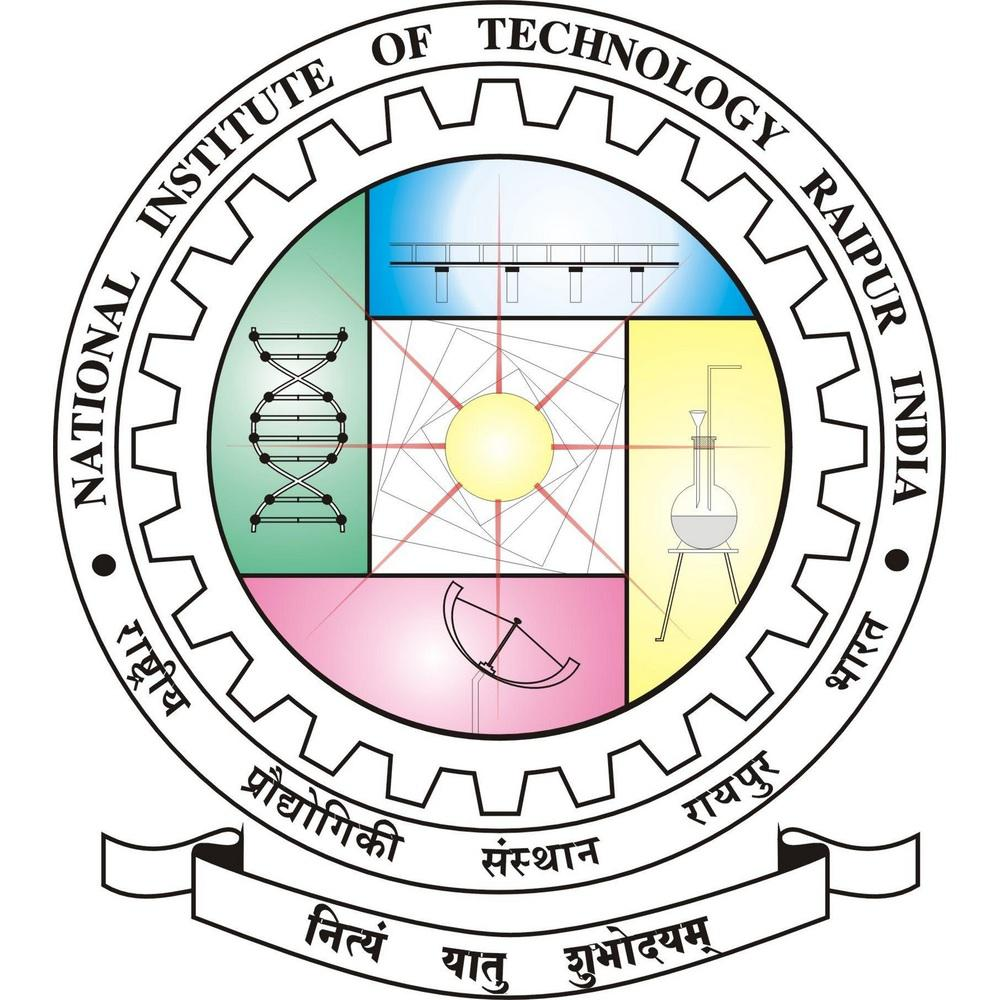
\includegraphics[scale = 0.20]{logo.jpeg}\\[1.0 cm]	% University Logo
    \textsc{\LARGE  National Institute of Technology\newline\newline Raipur}\\[2.0 cm]	% University Name
	\textsc{\Large assignment 02}\\[0.5 cm]				% Course Code
	\rule{\linewidth}{0.2 mm} \\[0.4 cm]
	{ \huge \bfseries \thetitle}\\
	\rule{\linewidth}{0.2 mm} \\[1.0 cm]
	
	\begin{minipage}{0.4\textwidth}
		\begin{flushleft} \large
			\emph{Submitted To:}\\
			Saurabh Gupta\\
            Asst. Professor\\
            Department of Biomedical Engineering\\
			\end{flushleft}
			\end{minipage}~
			\begin{minipage}{0.4\textwidth}
            
			\begin{flushright} \large
			\emph{Submitted By :} \\
			Naveen Choudhary\\
            21111034\\
        First Semester\\
        Biomedical Engineering\\
		\end{flushright}
        
	\end{minipage}\\[2 cm]
	

\end{titlepage}

\newpage

Medical technology has come a long way since the invention of eyeglasses and the stethoscope. The broader availability of mobile internet, the expansion of a more affluent middle class, and an aging global population are all driving change in the healthcare industry, and the associated technology is changing faster than ever before. Many of the most interesting new technologies in medicine need to be used together, and integrated attempts to do so already exist. Some tech-inspired clinics, such as Forward and One Medical, take a concierge-like approach to primary care, putting technology to use in a way that providers get more quality time with their patients. In 2020, the Covid-19 pandemic forced healthcare into the future, and, as a result, several promising medical technologies were tested on a massive scale. 

\indent

Telemedicine took a great leap forward during the Covid-19 pandemic. In January 2020, an estimated 24 percent of healthcare organizations had an existing telehealth program. For 2021, many healthcare organizations will be focusing on how best to integrate telehealth services with existing physical ones. Virtual visits will continue to be used as a way to increase access to primary care and urgent care, as well as to improve collaboration with clinics, long-term care facilities, dialysis centers, and mental health services. 

\indent

The development of multiple safe and effective Covid-19 vaccines in less than a year may be remembered as one of the greater scientific accomplishments in human history. The process was sped along not only by regulatory fast-tracking but also by innovations in the ways medical trials are conducted: virtual clinical trials, held mostly online, eased the burden of participation. Some of the relaxed regulatory procedures around drug development will fade with the Covid-19 pandemic, but innovative approaches to testing and collaboration could linger.

\indent

As the collection of health data continues to accelerate, its applications become more widespread, and its potential for improving treatment options and patient outcomes skyrockets. The biggest barrier, however, has been a lack of interoperability: one healthcare organization’s data is not easily transferred to (and easily processed by) another organization. Interoperability took a large step forward in November 2020, when Google Cloud launched its healthcare interoperability readiness program. Aimed at helping payers, providers, and other organizations prepare for the federal government’s interoperability regulations, it gives program participants access to data templates, app blueprints, security tools, and implementation guidelines.

\indent

Nanomedicine is the medical application of nanotechnology, the technology that operates on the atomic, molecular, or supramolecular scale. For something of such a small size, the potential is huge: nanomedicine has applications in imaging, sensing, diagnosis, and delivery through medical devices.If the biggest drivers of cutting-edge technology—AI, IoT, and Big Data—are to reach their full potential in healthcare, they need a reliable and lightning-fast internet connection. Enter 5G. With a reliable real-time connection, the most immediate benefits will be seen in telemedicine, expanding access to care for millions. But that’s only the beginning. More connected devices, with more authentic data streams, open up the possibility of a revolutionized healthcare system.

\indent

The artificial pacemaker, which dates back over 100 years, is still a critical piece of medical technology: over a million patients use them. By delivering electrical impulses to heart muscle chambers, they can prevent or correct life-threatening heart arrhythmias. Remotely monitoring these devices is an essential part of their functionality. Traditionally, that monitoring has been far from optimal, relying on complex interfaces that the patient may not fully understand. By enabling pacemakers with Bluetooth technology, they can be linked with smartphone-based mobile apps that patients better understand and utilize. That, in turn, improves remote monitoring, and, as a result, patient outcomes.

\indent

Fitness trackers have been on the rise for years. For diabetes patients, wearable continuous glucose monitors (CGMs) are set to become the new normal. Wearable CGMs remove the need for intermittent glucose testing and instead keep track of one’s blood sugar levels in real time. This allows users to see the immediate impacts of food and exercise, and shape their lifestyles accordingly. The healthcare systems have evolved a lot and yet many evolutions are to come. Engineers are still researching to make the complex healthcare system to a easy one. We are going to exerience a lot of innovations in the healthcare system.

\end{document}
